\subsubsection{Convection in a 2d box with a phase transition}
\label{sec:cookbooks-phase-function}

\textit{This section was contributed by Juliane Dannberg.}

This cookbook shows how to use a phase function formulation to introduce phase transitions in a model, using the setup of \cite{CY85} (which was the paper that originally introduced phase functions). The paper includes several different setups; here we only reproduce the incompressible cases using the Boussinesq Approximation.  

The model setup is a 2d quadratic box with prescribed temperatures at the top and bottom, insulating side walls, and free slip conditions on all boundaries. All material properties are constant, except for the density, which depends on temperature and on the stable phase. There is one phase transition in the center of the model domain (at a depth of 675 km), and the stable phase is represented by the phase function
\begin{equation}
  \Gamma = 0.5 \left(1 + \tanh \frac{p_h - \gamma T}{d \rho_0 g} \right), 
\end{equation}
which defines the fraction of the material that has already undergone the transition to the denser phase and takes the shape of a hyperbolic tangent. The phase function is 0 above the transition, and 1 below the transition. Here, $p_h$ is the hydrostatic pressure, $\gamma = -2.7~\si{\mega\pascal\per\kelvin}$ is the Clapeyron slope of the phase transition, $\rho_0 = 1000~\si{\kg\per\cubic\meter}$ is the reference density, $g = 10~\si{\metre\per\square\second}$ is the magnitude of the gravitational acceleration, and $d = 67.5~\si{\km}$ is the half-thickness of the phase transition (corresponding to 5\% of the height of the box). 

In the model series presented in \cite{CY85}, two important parameters are varied: the Rayleigh number (see for example Section~\ref{sec:cookbooks-simple-box}), which takes the values $Ra = 10^4$, $10^5$, $4 \times 10^5$ and $2 \times 10^6$, and the phase buoyancy parameter, which is controlled by the Clapeyron slope of the phase transition (see \cite{CY85}) and takes values between $-0.8$ and $0.4$. For a negative Clapeyron slope/phase buoyancy, the phase transition impedes flow; for a positive Clapeyron slope/phase buoyancy, the phase transition accelerates flow. 

In order to set up this model in \aspect{}, we use the latent heat material model, which includes an implementation of the phase function formulation. 
The model in \cite{CY85} is nondimensional, but we want to use Earth-like parameters here. To achieve this, we set most material properties to multiples of 10, and then control the three important model parameters by setting
\begin{enumerate}
  \item the thermal conductivity to $k = 2.460375 \times 10^7 / Ra~\si{\watt\per\metre\per\kelvin}$, to set the Rayleigh number,
  \item the Clapeyron slope to $\gamma = P (Ra/Rb) (\rho_0 g h/\Delta T) = P/2 \times 1.35 \times 10^7~\si{\pascal\per\kelvin}$ Pa/K, to set the phase buoyancy parameter $P$ (where $Rb$ is the boundary Rayleigh number, defined analogous to the Rayleigh number as $Rb = \Delta \rho g h^3 / \kappa \eta$, $h=1350~\si{\km}$ is the height of the box, and $\Delta T = 1000~\si{\kelvin}$ is the temperature difference between the top and bottom of the box), and 
  \item the density change across the phase transition to $\Delta \rho = 2 \alpha \rho_0 \Delta T = 200~\si{\kg\per\cubic\meter}$, to achieve $Rb$ = 2$Ra$ (where $\alpha = 10^{-4}~\si{\per\kelvin}$ is the thermal expansivity). 
\end{enumerate}   

Our input file is for a Rayleigh number of $Ra = 10^5$ and a phase buoyancy parameter of $P=-0.4$.                                  
The material properties are therefore set as follows:

\lstinputlisting[language=prmfile]{material.part.prm.out}

We run the model until a steady state heat flow is reached, or, in case the model does not reach steady state, until a time of 200 Myr. 
Depending on the Rayleigh number and the phase buoyancy parameter, the flow pattern in steady state can be very different: For positive or low negative Clapeyron slopes, one large convection cell develops. The more negative the Clapeyron slope of the phase transition, the more it impedes the flow, leading to episodic, or completely layered convection (see Figure~\ref{fig:christensen_yuen}). 

\begin{figure}
\centering
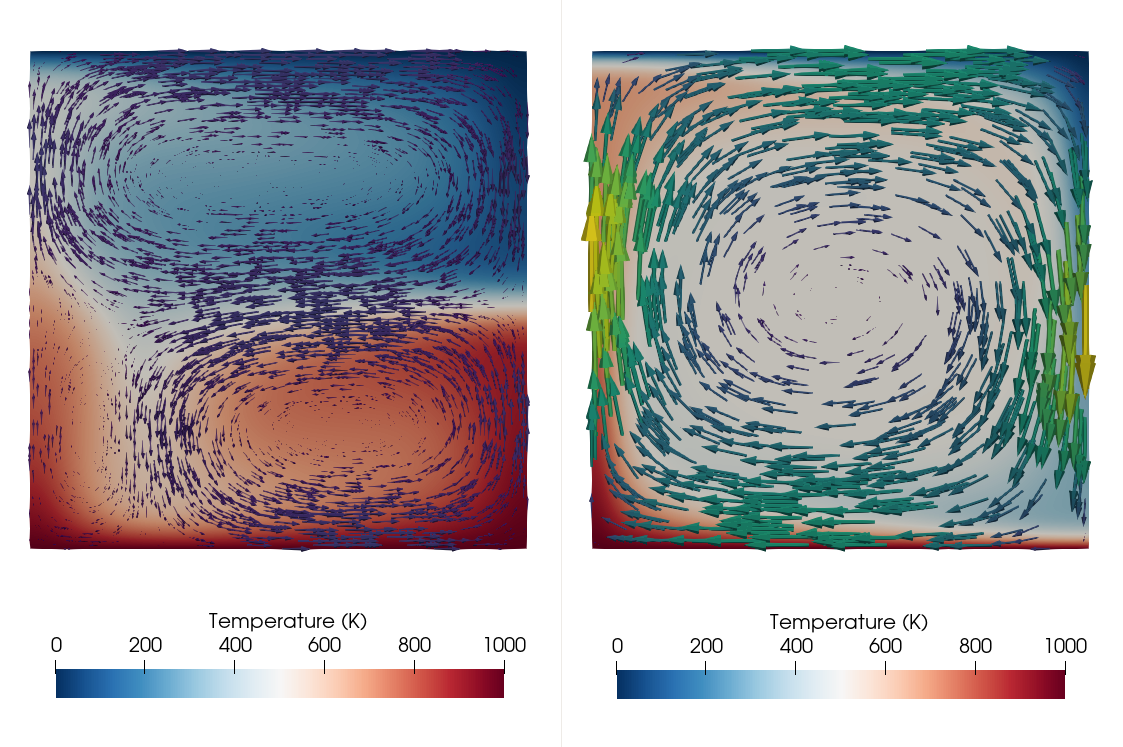
\includegraphics[width=0.8\textwidth]{flow_field.png}
\caption{\it Phase function model: Flow field in steady state for two models with a Rayleigh number of $Ra = 10^5$, but different phase buoyancy. The model on the left has a Clapeyron slope of $-2.7~\si{\mega\pascal\per\kelvin}$ (corresponding to $P=-0.4$) as in the original input file, leading to layered convection. The model on the right has a Clapeyron slope of $+2.7~\si{\mega\pascal\per\kelvin}$ (corresponding to $P=0.4$), leading to one large convection cell.}
\label{fig:christensen_yuen}
\end{figure}

The shell script \texttt{run\_all\_models.sh} in the same folder can be used to run the whole model series of Boussinesq cases presented in \cite{CY85}.  
